\documentclass[10pt, a4paper]{article}

\usepackage{ctex}
\usepackage{xeCJK}
\usepackage{caption}
\usepackage{geometry}
\geometry{
    left = 0.6in,
    right = 0.6in,
    top = 0.8in,
    bottom = 1.0in
}
\usepackage{amssymb}
\usepackage{amsbsy}
\usepackage{amsmath}
\usepackage{xcolor}
\usepackage{mathrsfs}
\usepackage{graphicx}
\usepackage{pifont}
\usepackage{tasks}
\settasks{
    label = \Alph*. ,
    label-width = 16pt
}
\pagestyle{empty}

\newcommand{\Title}[3]{
    \begin{center}
        \Large \textbf{中国电子学会 #1~年~#2~月 Scratch~#3级考试}
    \end{center}
}
\newcommand{\TimeAndName}[1]{
    \begin{center}
        考试时间:~#1~ 分钟 \qquad\qquad\qquad\qquad 姓名:\underline{\quad\quad\quad\quad}
    \end{center}
}

\begin{document}
    \Title{2022}{3}{二} % 标题
    \TimeAndName{60} % 考试时间及姓名

    % 单选题
    \vspace{2mm}
    {\noindent\textbf{第一部分、单选题(共 25 题,每题 2 分,共50分.)}}
    \begin{enumerate}
        % 1
        \item 红框中加入哪个选项积木,不能阻止气球下落?(\qquad)
        \begin{tasks}(4)
            \task 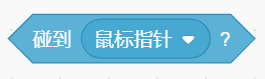
\includegraphics[width=.18\textwidth]{1a.png}
            \task 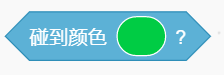
\includegraphics[width=.15\textwidth]{1b.png}
            \task 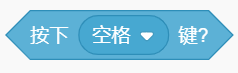
\includegraphics[width=.15\textwidth]{1c.png}
            \task 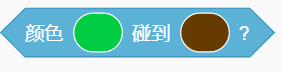
\includegraphics[width=.18\textwidth]{1d.png}
        \end{tasks}

        % 2
        \item 运行下列程序,会画出?(\qquad)
        \begin{tasks}(4)
            \task 一条横的实线
            \task 一条横的虚线
            \task 一条竖的实线
            \task 一条竖的虚线
        \end{tasks}

        \begin{figure}[htbp]
            \begin{minipage}[t]{.35\textwidth}
                \centering
                \begin{minipage}[t]{.5\textwidth}
                    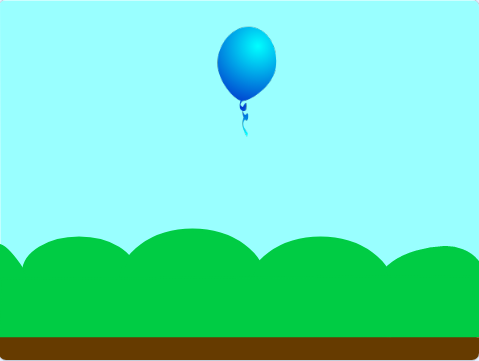
\includegraphics[width=\textwidth]{1-1.png}
                \end{minipage}
                \begin{minipage}[t]{.45\textwidth}
                    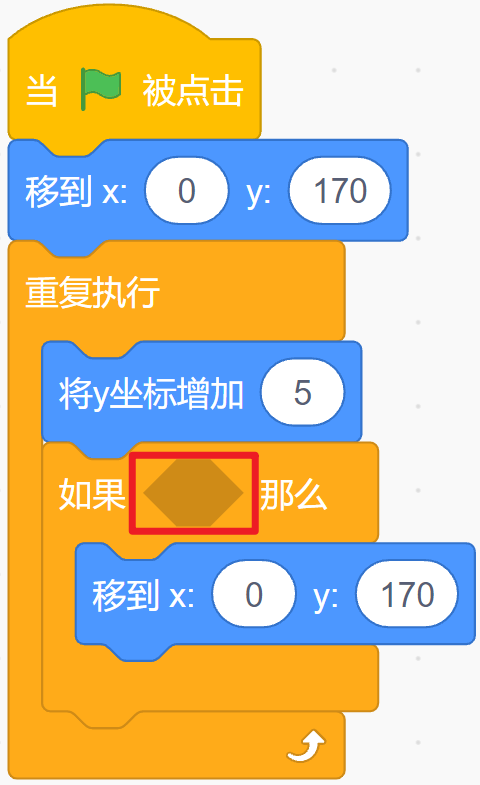
\includegraphics[width=\textwidth]{1-2.png}
                \end{minipage}
                \caption*{第 1 题}
            \end{minipage}
            \begin{minipage}[t]{.11\textwidth}
                \centering
                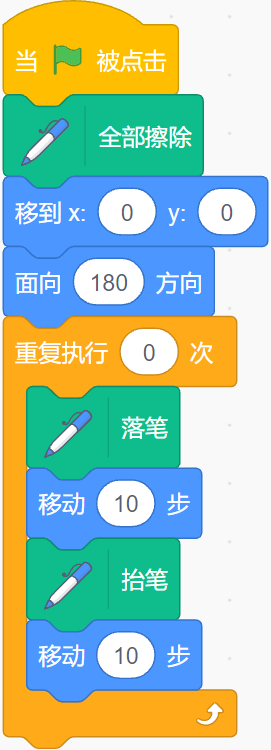
\includegraphics[width=\textwidth]{2.png}
                \caption*{第 2 题}
            \end{minipage}
            \begin{minipage}[t]{.2\textwidth}
                \centering
                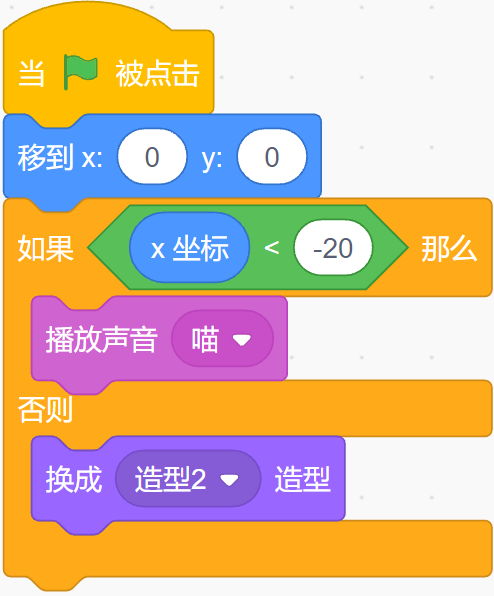
\includegraphics[width=\textwidth]{3.png}
                \caption*{第 3 题}
            \end{minipage}
            \begin{minipage}[t]{.32\textwidth}
                \centering
                \begin{minipage}[t]{.4\textwidth}
                    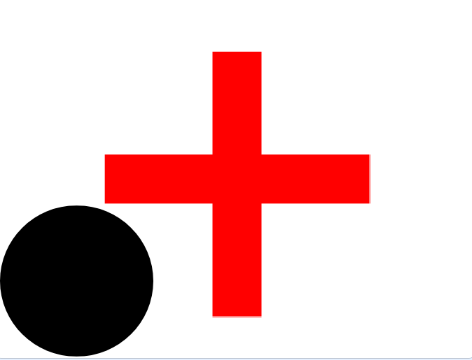
\includegraphics[width=\textwidth]{4-1.png}
                \end{minipage}
                \begin{minipage}[t]{.55\textwidth}
                    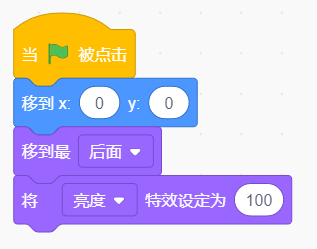
\includegraphics[width=\textwidth]{4-2.png}
                \end{minipage}
                \caption*{第 4 题}
            \end{minipage}
        \end{figure}

        % 3
        \item 如上图所示,默认小猫角色,点击绿旗后,下列哪个选项正确?(\qquad)
        \begin{tasks}(4)
            \task 小猫造型为造型1
            \task 小猫造型为造型2
            \task 小猫发出“喵”的声音
            \task 小猫无任何变化
        \end{tasks}

        % 4
        \item 上图分别是两个角色的初始位置和“黑色圆形”的程序,点击绿旗后,角色显示为下列哪个选项?(\qquad)
        \begin{tasks}(4)
            \task 
\includegraphics[width=.1\textwidth]{4a.png}
            \task 
\includegraphics[width=.1\textwidth]{4b.png}
            \task 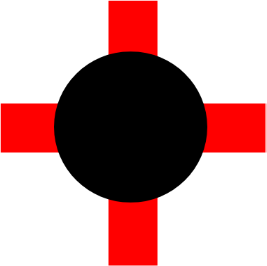
\includegraphics[width=.1\textwidth]{4c.png}
            \task 
\includegraphics[width=.1\textwidth]{4d.png}
        \end{tasks}

        % 5
        \item 默认小猫角色,点击绿旗后,下列哪个选项正确?(\qquad)
        
        \begin{minipage}{.3\textwidth}
            \centering
            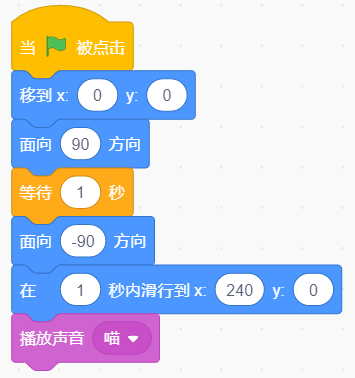
\includegraphics[width=.7\textwidth]{5.png}
        \end{minipage}
        \begin{minipage}{.64\textwidth}
            \begin{tasks}
                \task 1秒后滑行到舞台最右边,然后播放“喵”的声音
                \task 2秒后滑行到舞台最左边,然后播放“喵”的声音
                \task 1秒后滑行到舞台最左边,然后播放“喵”的声音
                \task 2秒后滑行到舞台最右边,然后播放“喵”的声音
            \end{tasks}
        \end{minipage}

        \newpage
        % 6
        \item 飞船程序如下图所示,点击绿旗后,按下空格键,下列哪个选项正确?(\qquad)
        \begin{tasks}(2)
            \task 飞船一直飞行,没有变化
            \task 飞船加速飞行
            \task 飞船隐身
            \task 飞船发生扭曲
        \end{tasks}

        % 7
        \item 默认小猫角色,点击绿旗后,按下空格键,角色的运行轨迹是?(\qquad)
        \begin{tasks}(2)
            \task 从中心处向左移动,再向上移动
            \task 从中心处向右移动,再向上移动
            \task 从中心处向左移动,再向下移动
            \task 从中心处向右移动,再向下移动
        \end{tasks}

        \begin{figure}[htbp]
            \centering
            \begin{minipage}[t]{.4\textwidth}
                \centering
                \begin{minipage}[t]{.48\textwidth}
                    \centering
                    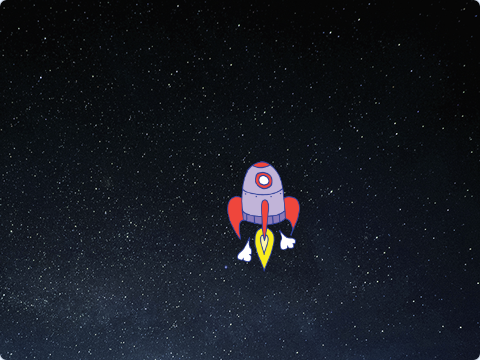
\includegraphics[width=\textwidth]{6-1.png}
                \end{minipage}
                \begin{minipage}[t]{.42\textwidth}
                    \centering
                    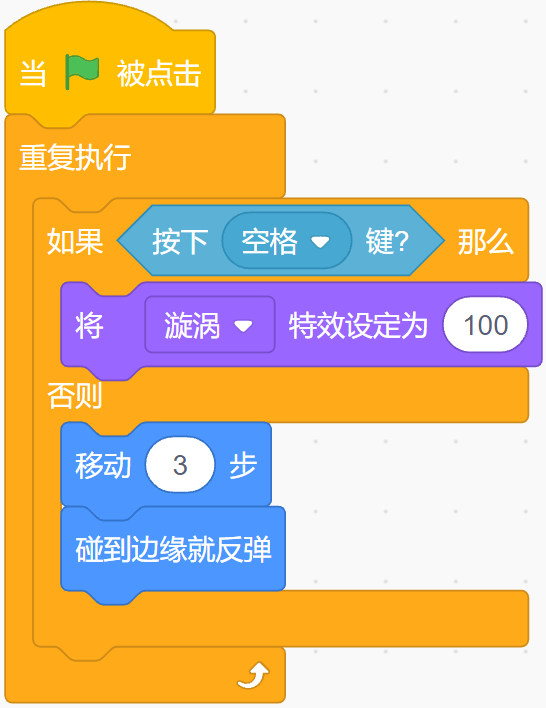
\includegraphics[width=\textwidth]{6-2.png}
                \end{minipage}
                \caption*{第 6 题}
            \end{minipage}
            \begin{minipage}[t]{.18\textwidth}
                \centering
                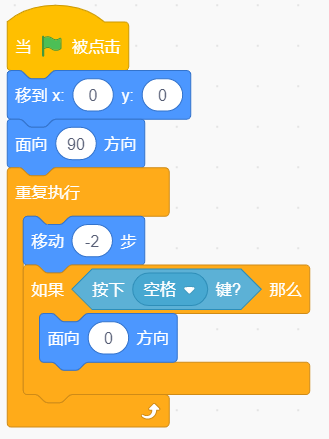
\includegraphics[width=\textwidth]{7.png}
                \caption*{第 7 题}
            \end{minipage}
            \begin{minipage}[t]{.25\textwidth}
                \centering
                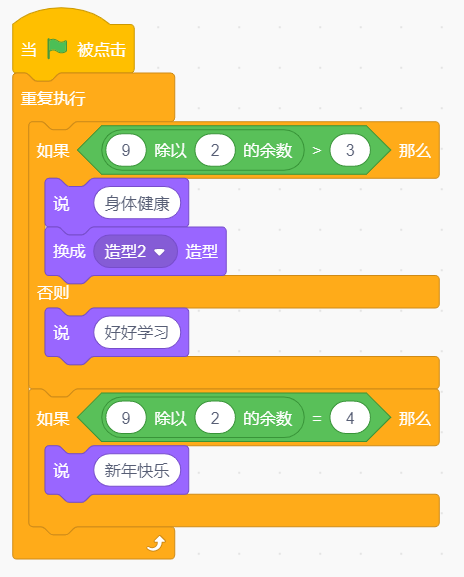
\includegraphics[width=\textwidth]{8.png}
                \caption*{第 8 题}
            \end{minipage}
        \end{figure}

        % 8
        \item 默认小猫角色,点击绿旗后,下列哪个选项正确?(\qquad)
        \begin{tasks}(4)
            \task 小猫说:身体健康
            \task 小猫说:好好学习
            \task 小猫说:新年快乐
            \task 小猫切换为“造型2”
        \end{tasks}

        % 9
        \item 找规律:数列 $1, 3, 4, 7, 11, (\quad)$, 括号的数是下列哪个选项?(\qquad)
        \begin{tasks}(4)
            \task 12
            \task 13
            \task 15
            \task 18
        \end{tasks}

        % 10
        \item 角色的初始状态如图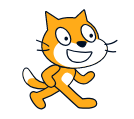
\includegraphics[width=.1\textwidth]{10.png}所示,以下积木的“特效”设置和角色所发生的变化不相符的是哪一个?(\qquad)
        \begin{tasks}(4)
            \task 
\includegraphics[width=.15\textwidth]{10a.png}
            \task 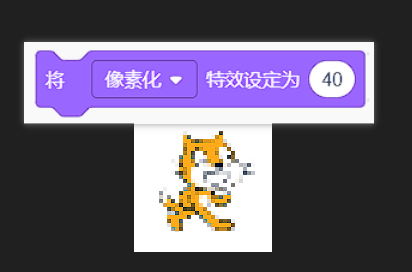
\includegraphics[width=.18\textwidth]{10b.png}
            \task 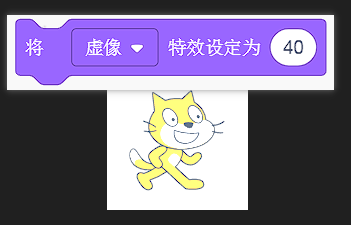
\includegraphics[width=.18\textwidth]{10c.png}
            \task 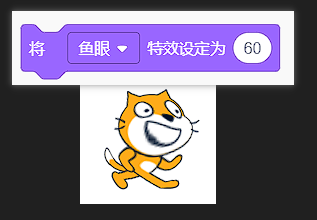
\includegraphics[width=.18\textwidth]{10d.png}
        \end{tasks}

        % 11
        \item 默认小猫角色,点击绿旗后,下列哪个选项正确?(\qquad)
        
        \begin{minipage}{.3\textwidth}
            \centering
            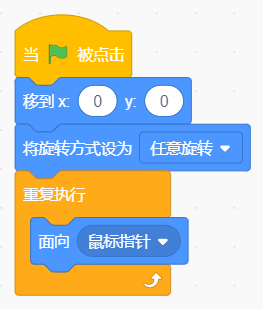
\includegraphics[width=.6\textwidth]{11.png}
        \end{minipage}
        \begin{minipage}{.6\textwidth}
            \begin{tasks}
                \task 角色的方向跟着鼠标改变,角色的位置不发生改变
                \task 角色的方向跟着鼠标改变,角色的位置会发生改变
                \task 角色跟着鼠标移动,角色的方向不会发生改变
                \task 角色跟着鼠标移动,角色的方向也跟着鼠标改变
            \end{tasks}
        \end{minipage}

        \newpage
        % 12
        \item 如下图所示,下面的流程图可以用哪个积木实现?(\qquad)
        \begin{tasks}(4)
            \task 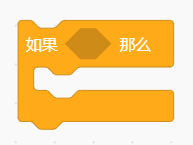
\includegraphics[width=.18\textwidth]{12a.png}
            \task 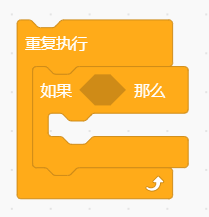
\includegraphics[width=.15\textwidth]{12b.png}
            \task 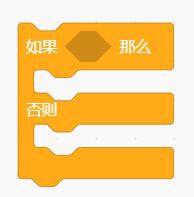
\includegraphics[width=.15\textwidth]{12c.png}
            \task 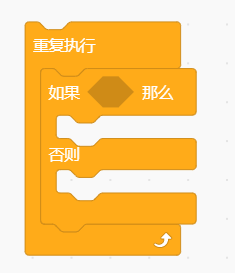
\includegraphics[width=.15\textwidth]{12d.png}
        \end{tasks}

        % 13
        \item 如下图所示,下列程序空白处填写哪个选项,可以让角色播放声音:“体温异常”?(\qquad)
        \begin{tasks}(4)
            \task 37.5
            \task 37.3
            \task 37.0
            \task 36.8
        \end{tasks}
        
        \begin{figure}[htbp]
            \centering
            \begin{minipage}[t]{.2\textwidth}
                \centering
                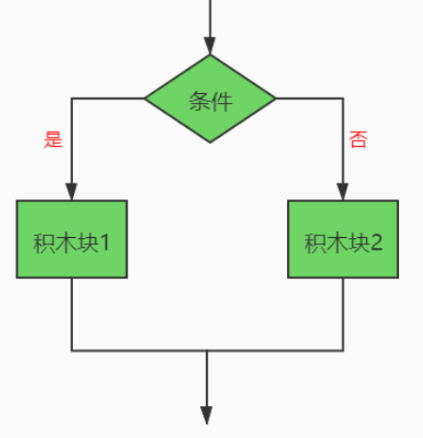
\includegraphics[width=\textwidth]{12.png}
                \caption*{第 12 题}
            \end{minipage}
            \begin{minipage}[t]{.2\textwidth}
                \centering
                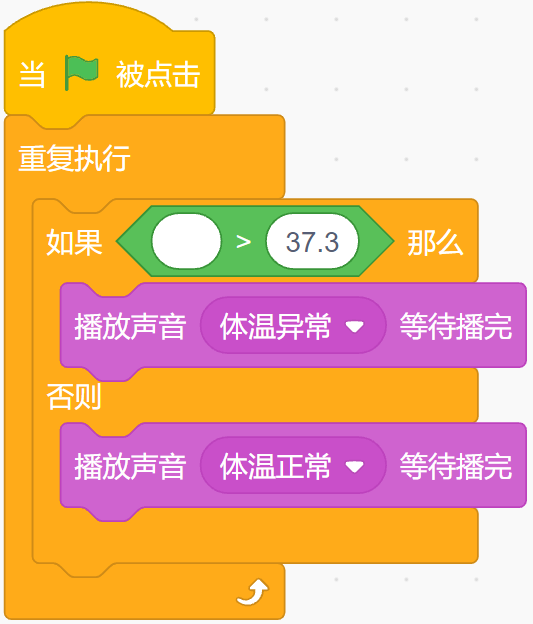
\includegraphics[width=\textwidth]{13.png}
                \caption*{第 13 题}
            \end{minipage}
            \begin{minipage}[t]{.33\textwidth}
                \centering
                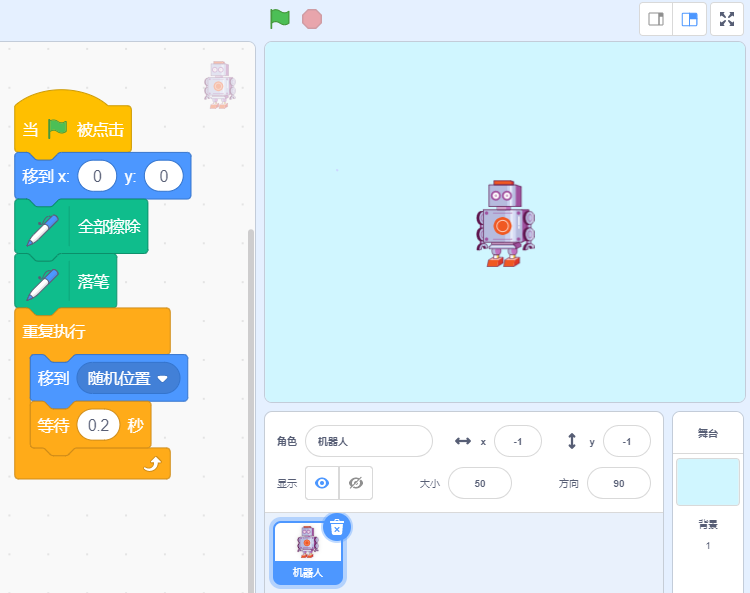
\includegraphics[width=\textwidth]{14.png}
                \caption*{第 14 题}
            \end{minipage}
        \end{figure}

        % 14
        \item 如上图所示,点击绿旗后,下列哪个选项正确?(\qquad)
        \begin{tasks}(2)
            \task 每次单击绿旗,机器人画出的图形都相同。
            \task 每次单击绿旗,机器人画出的图形可能是不同的
            \task 单击绿旗后,机器人会一直移动,但不会画出图形
            \task 单击绿旗后,机器人移动,碰到边缘就不动了
        \end{tasks}

        % 15
        \item 如下图所示,下列哪个选项能够让音乐在播放时声音越来越小?(\qquad)
        \begin{tasks}(4)
            \task 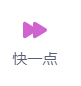
\includegraphics[width=.05\textwidth]{15a.png}
            \task 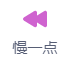
\includegraphics[width=.05\textwidth]{15b.png}
            \task 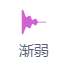
\includegraphics[width=.05\textwidth]{15c.png}
            \task 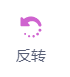
\includegraphics[width=.05\textwidth]{15d.png}
        \end{tasks}

        \begin{figure}[htbp]
            \centering
            \begin{minipage}[t]{.45\textwidth}
                \centering
                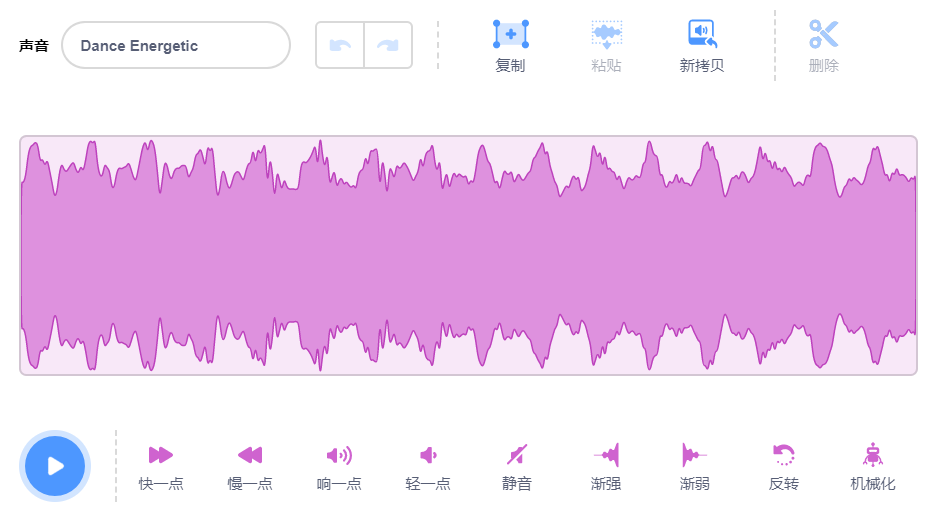
\includegraphics[width=\textwidth]{15.png}
                \caption*{第 15 题}
            \end{minipage}
            \begin{minipage}[t]{.5\textwidth}
                \centering
                \begin{minipage}[t]{.35\textwidth}
                    \centering
                    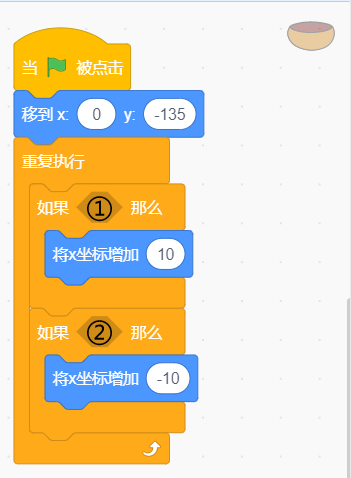
\includegraphics[width=\textwidth]{16-1.png}
                \end{minipage}
                \begin{minipage}[t]{.43\textwidth}
                    \centering
                    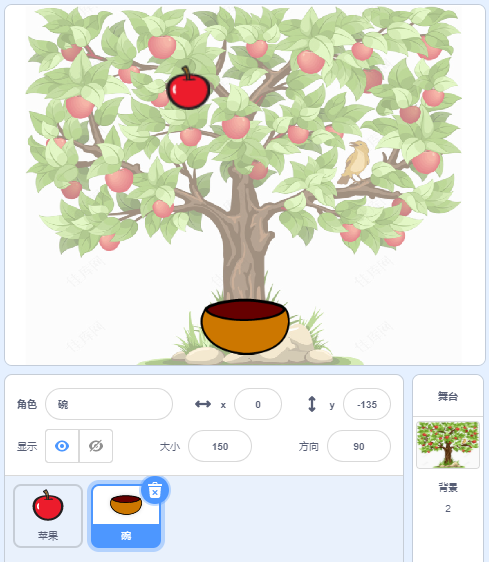
\includegraphics[width=\textwidth]{16-2.png}
                \end{minipage}
                \caption*{第 16 题}
            \end{minipage}
        \end{figure}

        % 16
        \item 如上图所示,按下左右键控制角色左右移动,\ding{172} 和 \ding{173} 处应该填入哪个选项?(\qquad)
        \begin{tasks}(2)
            \task 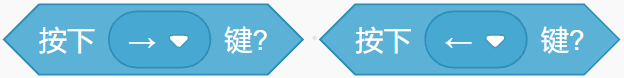
\includegraphics[width=.3\textwidth]{16a.png}
            \task 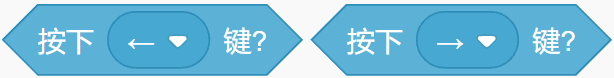
\includegraphics[width=.3\textwidth]{16b.png}
            \task 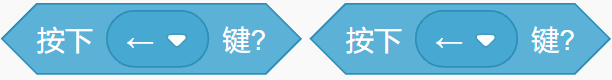
\includegraphics[width=.3\textwidth]{16c.png}
            \task 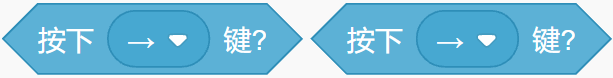
\includegraphics[width=.3\textwidth]{16d.png}
        \end{tasks}

        \newpage
        % 17
        \item 看图 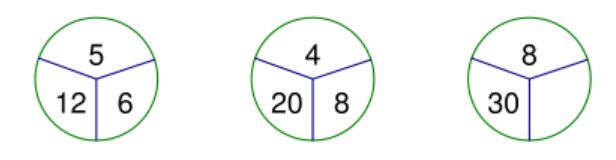
\includegraphics[width=.25\textwidth]{17.png} 找规律:第三个图形的空白处应填什么数?(\qquad)
        \begin{tasks}(4)
            \task 12
            \task 15
            \task 24
            \task 26
        \end{tasks}

        % 18
        \item 下图是钟表表盘和秒针,给秒针编程,下列哪个选项正确?(\qquad)
        \begin{tasks}(4)
            \task 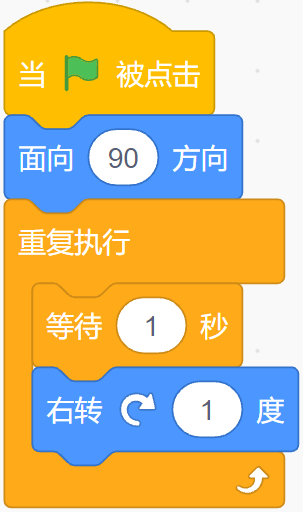
\includegraphics[width=.12\textwidth]{18a.png}
            \task 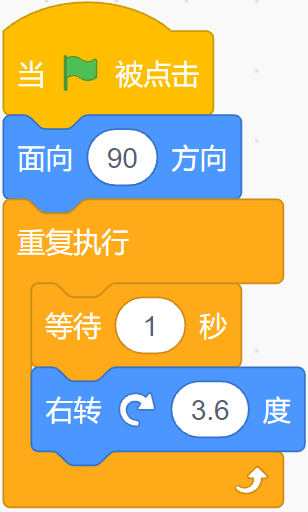
\includegraphics[width=.12\textwidth]{18b.png}
            \task 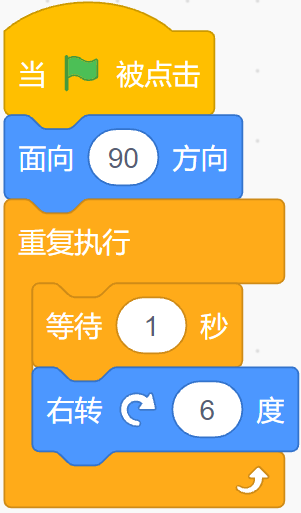
\includegraphics[width=.12\textwidth]{18c.png}
            \task 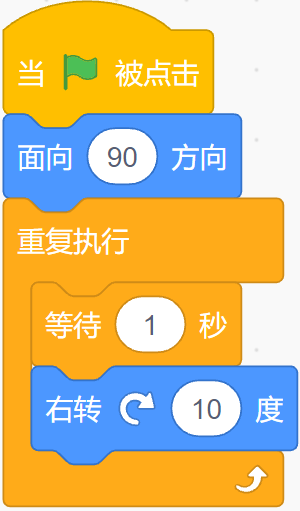
\includegraphics[width=.12\textwidth]{18d.png}
        \end{tasks}

        % 19
        \item 积木块 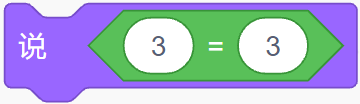
\includegraphics[width=.15\textwidth]{19.png} 的执行结果是?(\qquad)
        \begin{tasks}(4)
            \task 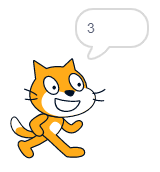
\includegraphics[width=.12\textwidth]{19a.png}
            \task \includegraphics[width=.12\textwidth]{19b.png}
            \task \includegraphics[width=.12\textwidth]{19c.png}
            \task \includegraphics[width=.12\textwidth]{19d.png}
        \end{tasks}

        \begin{figure}[htbp]
            \centering
            \begin{minipage}[t]{.15\textwidth}
                \centering
                \includegraphics[width=\textwidth]{18.jpg}
                \caption*{第 18 题}
            \end{minipage}
            \begin{minipage}[t]{.15\textwidth}
                \centering
                \includegraphics[width=\textwidth]{21.png}
                \caption*{第 21 题}
            \end{minipage}
            \begin{minipage}[t]{.42\textwidth}
                \centering
                \includegraphics[width=\textwidth]{22.png}
                \caption*{第 22 题}
            \end{minipage}
        \end{figure}

        % 20
        \item 下列哪个积木不能实现循环功能?(\qquad)
        \begin{tasks}(4)
            \task \includegraphics[width=.14\textwidth]{20a.png}
            \task \includegraphics[width=.12\textwidth]{20b.png}
            \task \includegraphics[width=.12\textwidth]{20c.png}
            \task \includegraphics[width=.12\textwidth]{20d.png}
        \end{tasks}

        % 21
        \item 如上图所示.关于下列积木,说法正确的是?(\qquad)
        \begin{tasks}(2)
            \task 当条件满足时,执行红框内积木
            \task 它是条件循环积木
            \task 是有限循环,不能无限循环
            \task 红框内积木一定会被执行
        \end{tasks}

        % 22
        \item 上图程序运行的结果是?(\qquad)
        \begin{tasks}(4)
            \task pa
            \task py
            \task ph
            \task pl
        \end{tasks}

        % 23
        \item 下列哪个积木运行结果是false?(\qquad)
        \begin{tasks}(2)
            \task \includegraphics[width=.2\textwidth]{23a.png}
            \task \includegraphics[width=.15\textwidth]{23b.png}
            \task \includegraphics[width=.2\textwidth]{23c.png}
            \task \includegraphics[width=.2\textwidth]{23d.png}
        \end{tasks}

        \newpage
        % 24
        \item 三位小朋友比年龄大小,根据下面三句话,谁最大,谁最小?(\qquad)
        
        \ding{172}~小芳比小阳大3岁;

        \ding{173}~小燕比小芳小1岁;

        \ding{174}~小燕比小阳大2岁
        \begin{tasks}(4)
            \task 小燕最大,小阳最小
            \task 小芳最大,小阳最小
            \task 小芳最大,小燕最小
            \task 小阳最大,小燕最小
        \end{tasks}

        % 25
        \item 看图 \includegraphics[width=.25\textwidth]{25.png} 找规律:$a$ 和 $b$ 的值是多少?(\qquad)
        \begin{tasks}(4)
            \task 35, 5
            \task 36, 5
            \task 38, 6
            \task 39, 7
        \end{tasks}
    \end{enumerate}

    % \begin{figure}[htbp]
    %     \centering
    %     \begin{minipage}[t]{.15\textwidth}
    %         \centering
    %         \includegraphics[width=\textwidth]{24.png}
    %         \caption*{第 24 题}
    %     \end{minipage}
    %     \begin{minipage}[t]{.14\textwidth}
    %         \centering
    %         \includegraphics[width=\textwidth]{25.png}
    %         \caption*{第 25 题}
    %     \end{minipage}
    %     \begin{minipage}[t]{.29\textwidth}
    %         \begin{minipage}[t]{.45\textwidth}
    %             \centering
    %             \includegraphics[width=\textwidth]{26-1.png}
    %         \end{minipage}
    %         \begin{minipage}[t]{.53\textwidth}
    %             \centering
    %             \includegraphics[width=\textwidth]{26-2.png}
    %         \end{minipage}
    %         \caption*{第 26 题}
    %     \end{minipage}
    %     \begin{minipage}[t]{.23\textwidth}
    %         \centering
    %         \includegraphics[width=\textwidth]{27.png}
    %         \caption*{第 27 题}
    %     \end{minipage}
    % \end{figure}

    % 判断题
    {\noindent\textbf{第二部分、判断题(共 10 题,每题 2 分,共20分.)}}
    \begin{enumerate}
        \setcounter{enumi}{25}
        % 26
        \item 如图所示 \includegraphics[width=.12\textwidth]{26.png} 积木只能将声音音量调大. (\qquad)

        % 27
        \item 如下图所示,默认小猫角色,点击绿旗后,按下空格键,小猫会一直移动;不按空格键,小猫停止移动. (\qquad)

        % 28
        \item 如下图所示,默认小猫角色,点击小猫,小猫立即消失. (\qquad)

        % 29
        \item 红红、聪聪和颖颖都戴着太阳帽去参加野炊活动,她们的帽子分别是红的、黄的、蓝的,只知道红红没有戴黄帽子,聪聪既不戴黄帽子,也不戴蓝帽子。分析可知,红红戴的帽子是蓝色的. (\qquad)

        \begin{figure}[htbp]
            \centering
            \begin{minipage}[t]{.2\textwidth}
                \centering
                \includegraphics[width=\textwidth]{27.png}
                \caption*{第 27 题}
            \end{minipage}
            \begin{minipage}[t]{.19\textwidth}
                \centering
                \includegraphics[width=\textwidth]{28.png}
                \caption*{第 28 题}
            \end{minipage}
            \begin{minipage}[t]{.4\textwidth}
                \centering
                \includegraphics[width=\textwidth]{30.png}
                \caption*{第 30 题}
            \end{minipage}
        \end{figure}

        % 30
        \item 如上图所示,点击绿旗后,每次按下空格键,角色都会向上移动. (\qquad)

        % 31
        \item 如上图所示,小猫角色使用图章,小狗角色使用落笔和移动,绘制出如下的图案。使用“全部擦除”只能擦除小狗绘制出的图案. (\qquad)
        
        \begin{figure}[htbp]
            \centering
            \begin{minipage}[t]{.2\textwidth}
                \centering
                \includegraphics[width=\textwidth]{31.png}
                \caption*{第 31 题}
            \end{minipage}
            \begin{minipage}[t]{.35\textwidth}
                \centering
                \includegraphics[width=\textwidth]{32.png}
                \caption*{第 32 题}
            \end{minipage}
        \end{figure}

        % 32
        \item 声音“Alert”的时长为1.01秒,下列两段程序执行的效果一样. (\qquad)

        \newpage
        % 33
        \item 运行下列程序后,舞台区会出现3条线段. (\qquad)
        
        \begin{figure}[htbp]
            \centering
            \begin{minipage}[t]{.1\textwidth}
                \centering
                \includegraphics[width=\textwidth]{33.png}
                \caption*{第 33 题}
            \end{minipage}
            \begin{minipage}[t]{.45\textwidth}
                \centering
                \begin{minipage}[t]{.48\textwidth}
                    \centering
                    \includegraphics[width=\textwidth]{34-1.png}
                \end{minipage}
                \begin{minipage}[t]{.48\textwidth}
                    \centering
                    \includegraphics[width=\textwidth]{34-2.png}
                \end{minipage}
                \caption*{第 34 题}
            \end{minipage}
            \begin{minipage}[t]{.35\textwidth}
                \centering
                \begin{minipage}[t]{.48\textwidth}
                    \centering
                    \includegraphics[width=\textwidth]{35-1.png}
                \end{minipage}
                \begin{minipage}[t]{.48\textwidth}
                    \centering
                    \includegraphics[width=\textwidth]{35-2.png}
                \end{minipage}
                \caption*{第 35 题}
            \end{minipage}
        \end{figure}
        
        % 34
        \item 如上图所示,山洞的坐标为 $(155, 1)$,小熊执行下列程序后一定能回到山洞. (\qquad)

        % 35
        \item 小鸡初始位置和程序如上图所示,点击绿旗后,小鸡会越来越接近煌虫. (\qquad)
    \end{enumerate}

    {\noindent \textbf{第三部分、编程题(共 2 题,共30分.)}}
    \begin{enumerate}
        \setcounter{enumi}{35}
        
        % 36
        \item 魔法星空:
        
        1. 准备工作
        \begin{tasks}[label = (\arabic*)]
            \task 导入背景:Stars;
            \task 保留小猫角色;
            \task 导入声音"Emotional Piano"和"Jump"。
        \end{tasks}
        2. 功能实现
        \begin{tasks}[label = (\arabic*)]
            \task 程序开始,小猫隐藏,画笔的颜色设为红色,粗细设为20;
            \task 程序开始后,一直播放背景音乐“Emotional Piano";
            \task 按下空格键,播放声音Jump,画笔颜色增加10,在舞台的随机位置画出圆点;
            \task 当按下“$\to$”键,将笔的粗细增加5;
            \task 当按下“$\leftarrow$”键,将笔的粗细减小5。
        \end{tasks}
        \begin{figure}[htbp]
            \centering
            \includegraphics[width=.3\textwidth]{36.png}
        \end{figure}

        \newpage
        %37
        \item 跳跃游戏:
        
        1. 准备工作
        \begin{tasks}[label = (\arabic*)]
            \task 保留小猫角色,导入角色“Dog1”,调整小狗大小;
            \task 选择背景"Blue Sky"。
        \end{tasks}
        2. 功能实现
        \begin{tasks}[label = (\arabic*)]
            \task 小猫初始位置如上面第一张图所示;
            \task 点击绿旗后,小狗从舞台最右边跑到最左边后,再移到最右边,从最右边跑到最左边,一直执行下去;
            \task 按下空格键,小猫向上跳起一段距离后,又落到地面;
            \task 小猫碰到小狗,程序停止。
        \end{tasks}
        \begin{figure}[htbp]
            \centering
            \begin{minipage}[t]{.24\textwidth}
                \centering
                \includegraphics[width=\textwidth]{37-1.png}
            \end{minipage}
            \begin{minipage}[t]{.24\textwidth}
                \centering
                \includegraphics[width=\textwidth]{37-2.png}
            \end{minipage}
            \begin{minipage}[t]{.24\textwidth}
                \centering
                \includegraphics[width=\textwidth]{37-3.png}
            \end{minipage}
            \begin{minipage}[t]{.24\textwidth}
                \centering
                \includegraphics[width=\textwidth]{37-4.png}
            \end{minipage}
        \end{figure}
    \end{enumerate}
\end{document}